\documentclass[12pt]{article}
\usepackage{amsmath,amsfonts,amsthm,amssymb}
\usepackage{setspace}
\usepackage{fancyhdr}
\usepackage{lastpage}
\usepackage{extramarks}
\usepackage[ruled,vlined]{algorithm2e}
\usepackage{chngpage}
\usepackage{soul,color, xcolor}
\usepackage{graphicx,float,wrapfig}
\usepackage{ listings}
\usepackage{enumitem}
\usepackage{tikz}
\newcommand{\Class}{ \normalsize CS 331: Algorithms and Complexity (Spring 2024)\\
\small    Unique Number: 50930, 50935 50940, 50945
}


\newenvironment{solution}{
    \color{blue} \textbf{Solution:}
    }
    %\newcommand{\ClassInstructor}{Fares}

        \def\changemargin#1#2{\list{}{\rightmargin#2\leftmargin#1}\item[]}
\let\endchangemargin=\endlist
% Homework Specific Information. Change it to your own
\newcommand{\Title}{Assignment 3 - Solution}
\newcommand{\DueDate}{Thursday, 8 Febrauary, by 11.59pm}
\newcommand{\StudentName}{}
\newcommand{\StudentClass}{}
\newcommand{\StudentNumber}{}

% In case you need to adjust margins:
\topmargin=-0.45in      %
\evensidemargin=0in     %
\oddsidemargin=0in      %
\textwidth=6.5in        %
\textheight=9.0in       %
\headsep=0.25in         %

% Setup the header and footer
\pagestyle{fancy}                                                       %
\lhead{\StudentName}                                                 %
\chead{\Title}  %
\rhead{\firstxmark}                                                     %
\lfoot{\lastxmark}                                                      %
\cfoot{}                                                                %
\rfoot{Page\ \thepage\ of\ \protect\pageref{LastPage}}                          %
\renewcommand\headrulewidth{0.4pt}                                      %
\renewcommand\footrulewidth{0.4pt}                                      %

%%%%%%%%%%%%%%%%%%%%%%%%%%%%%%%%%%%%%%%%%%%%%%%%%%%%%%%%%%%%%
% Some tools
\newcommand{\enterProblemHeader}[1]{\nobreak\extramarks{#1}{#1 continued on next page\ldots}\nobreak%
\nobreak\extramarks{#1 (continued)}{#1 continued on next page\ldots}\nobreak}%
\newcommand{\exitProblemHeader}[1]{\nobreak\extramarks{#1 (continued)}{#1 continued on next page
\ldots}\nobreak%
\nobreak\extramarks{#1}{}\nobreak}%

\newcommand{\homeworkProblemName}{}%
\newcounter{homeworkProblemCounter}%
\newenvironment{homeworkProblem}[1][Problem \arabic{homeworkProblemCounter}]%
{\stepcounter{homeworkProblemCounter}%
\renewcommand{\homeworkProblemName}{#1}%
\section*{\homeworkProblemName}%
\enterProblemHeader{\homeworkProblemName}}%
{\exitProblemHeader{\homeworkProblemName}}%

\newcommand{\homeworkSectionName}{}%
\newlength{\homeworkSectionLabelLength}{}%
\newenvironment{homeworkSection}[1]%
{% We put this space here to make sure we're not connected to the above.

    \renewcommand{\homeworkSectionName}{#1}%
    \settowidth{\homeworkSectionLabelLength}{\homeworkSectionName}%
    \addtolength{\homeworkSectionLabelLength}{0.25in}%
    \changetext{}{-\homeworkSectionLabelLength}{}{}{}%
    \subsection*{\homeworkSectionName}%
    \enterProblemHeader{\homeworkProblemName\ [\homeworkSectionName]}}%
    {\enterProblemHeader{\homeworkProblemName}%

    % We put the blank space above in order to make sure this margin
    % change doesn't happen too soon.
    \changetext{}{+\homeworkSectionLabelLength}{}{}{}}%

\newcommand{\Answer}{\ \\\textbf{Answer:} }
\newcommand{\Acknowledgement}[1]{\ \\{\bf Acknowledgement:} #1}

%%%%%%%%%%%%%%%%%%%%%%%%%%%%%%%%%%%%%%%%%%%%%%%%%%%%%%%%%%%%%


%%%%%%%%%%%%%%%%%%%%%%%%%%%%%%%%%%%%%%%%%%%%%%%%%%%%%%%%%%%%%
% Make title
\newcommand{\maxpt}[1]{\ifthenelse{\equal{#1}{1}}{\textbf{(#1 pt)}}{\textbf{(#1 pts)}}}
\def \solcolor{blue}
\title{\textmd{\bf \Class\\ \Title}\\\vspace{0.1in}\small{Due\ on\ \DueDate}}
\date{}
\author{\textbf{\StudentName}\ \ \StudentClass\ \ \StudentNumber}
%%%%%%%%%%%%%%%%%%%%%%%%%%%%%%%%%%%%%%%%%%%%%%%%%%%%%%%%%%%%%

\begin{document}
    \maketitle \thispagestyle{empty}

    %        \begin{figure}[h]
    %            \centering
    %            \includegraphics[width=0.75\textwidth]{../HonorCode}
    %        \end{figure}


    %%%%%%%%%%%%%%%%%%%%%%%%%%%%%%%%%%%%%%%%%%%%%%%%%%%%%%%%%%%%%
    % Begin edit from here


    \def\changemargin#1#2{\list{}{\rightmargin#2\leftmargin#1}\item[]}
    \let\endchangemargin=\endlist

    \begin{homeworkProblem}[Problem 1: Short Answer Section]
        \maxpt{10} True or false. If true, briefly justify, otherwise, provide a counter example
        . When justifying, restrict answers to no more than a few sentences.
        \begin{enumerate}
            \item \maxpt{1}
            True, a greedy option picks the best option at each step, without considering the
            future.
            \item \maxpt{2}
            True, you argue that the differences between the two algorithms are irrelevant to the
            quality of the solution.
            \item \maxpt{2}
            True, since the shortest path is the path with the fewest edges.
            \item \maxpt{2}
            False, Counterexample:
            \begin{verbatim}
(1, 4), (4, 7), (3, 5), (3, 5)
Try (1, 4), but it has 2 conflicts, so discard it
Try (4, 7), but it has 2 conflicts, so discard it
Pick (3, 5), and since (1, 4) and (4, 7) are discarded, it has only one conflict
Then, our solution yields one job
However, the optimal solution is to pick (1, 4) and (4, 7)
            \end{verbatim}
            \item \maxpt{3}
            No, the shortest path is not necessarily the path with the fewest edges, Counterexample:
            \begin{verbatim}
(a, b) = 1; (b, c) = 1; (c, d) = 1; (a, d) = 4
Shortest path: a -> b -> c -> d with weight 3
Increment all edges by 1, we get: a -> b -> c -> d with weight 6
However, the shortest path is a -> d with weight 5
            \end{verbatim}
        \end{enumerate}
    \end{homeworkProblem}

    \begin{homeworkProblem}
        \textbf{(10 points)}
        I will denote tasks as (p(i), t(i)) where p(i) is the value of the task and t(i) is the
        duration of the task.
        \begin{enumerate}
            \item (Smallest duration first) Pick task $i$ that has the minimum duration $t(i)$, or
            \begin{proof}
                This is not optimal.\newline
                Counterexample:
                \begin{verbatim}
(1, 1), (10, 2)
Pick (1, 1) first, then (10, 2)
This yields (1 * 1) + (10 * 3) = 31
However, the optimal solution is to pick (10, 2) first, then (1, 1)
This yields (10 * 2) + (1 * 3) = 23
                \end{verbatim}
            \end{proof}
            \item (Most valuable first) Pick task $i$ that has maximum $p(i)$, or
            \begin{proof}
                This is not optimal.\newline
                Counterexample:
                \begin{verbatim}
(1, 1), (2, 3)
Pick (2, 3) first, then (1, 1)
This yields (2 * 3) + (1 * 4) = 10
However, the optimal solution is to pick (1, 1) first, then (2, 3)
This yields (1 * 1) + (2 * 4) = 9
                \end{verbatim}
            \end{proof}
            \item (Maximum time-scaled value first) Pick task $i$ that has maximum $p(i)/t(i)$.
            \begin{proof}
                This is optimal.\newline
                I will prove this using the exchange argument.\newline
                Let the optimal solution $\mathbb{O} = (o_1, o_2, \ldots, o_n)$ be the sequence of
                tasks that minimizes the total value.\newline
                Let the greedy solution $\mathbb{G} = (g_1, g_2, \ldots, g_n)$ be the greedy
                solution where we pick the task with the maximum $p(i)/t(i)$ first.\newline
                Assume there are tasks $(o_i, o_j)$ in $\mathbb{O}$ that is out of order in $\mathbb{G}$
                .\newline
                We can also assume they're consecutive in $\mathbb{O}$, since we can just
                iteratively swap consecutive tasks.\newline
                $\therefore$, we have to show the greedy solution doesn't increase the total
                value of the tasks after swapping them.\newline
                These two tasks have penalty $p(o_i) \cdot t(o_i) + p(o_j) \cdot (t(o_i) + t(o_j))$
                in $\mathbb{O}$.\newline
                We can expand this to $p(o_i) \cdot t(o_i) + p(o_j) \cdot t(o_i) + p(o_j) \cdot t(
                o_j)$.\newline
                After swapping them, the penalty becomes $p(o_j) \cdot t(o_j) + p(o_i) \cdot (t(o_i)
                + t(o_j))$.\newline
                We can expand this to $p(o_j) \cdot t(o_j) + p(o_i) \cdot t(o_i) + p(o_i) \cdot t(
                o_j)$.\newline
                Now we compare $p(o_i) \cdot t(o_i) + p(o_j) \cdot t(o_i) + p(o_j) \cdot t(
                o_j)$ \textquestiondown\;$p(o_j) \cdot t(o_j) + p(o_i) \cdot t(o_i) + p(o_i) \cdot t(
                o_j)$.\newline
                We can subtract $p(o_i) \cdot t(o_i)$ and $p(o_j) \cdot t(o_j)$ from both sides
                to get $p(o_j) \cdot t(o_i)$ \textquestiondown\;$p(o_i) \cdot t(o_j)$.\newline
                Divide both sides by $t(o_i) \cdot t(o_j)$ to get $\frac{p(o_j)}{t(o_j)}$ \textquestiondown\;$\frac{p(o_i)}{t(o_i)}$.\newline
                Then, by definition of $\mathbb{G}$, $\frac{p(o_j)}{t(o_j)} \geq \frac{p(o_i)}{t(
                    o_i)}$ since $o_j$ was before $o_i$ in the greedy solution.\newline
                $\therefore$, the optimal solution $\geq$ the greedy solution.\newline
                $\therefore$, the greedy solution is optimal.
            \end{proof}
        \end{enumerate}
    \end{homeworkProblem}

    \begin{homeworkProblem}
        \textbf{(10 points)}
        Yes, unless the graph has edges of equal weight with equal path weight and length from start
        to target node.\newline
        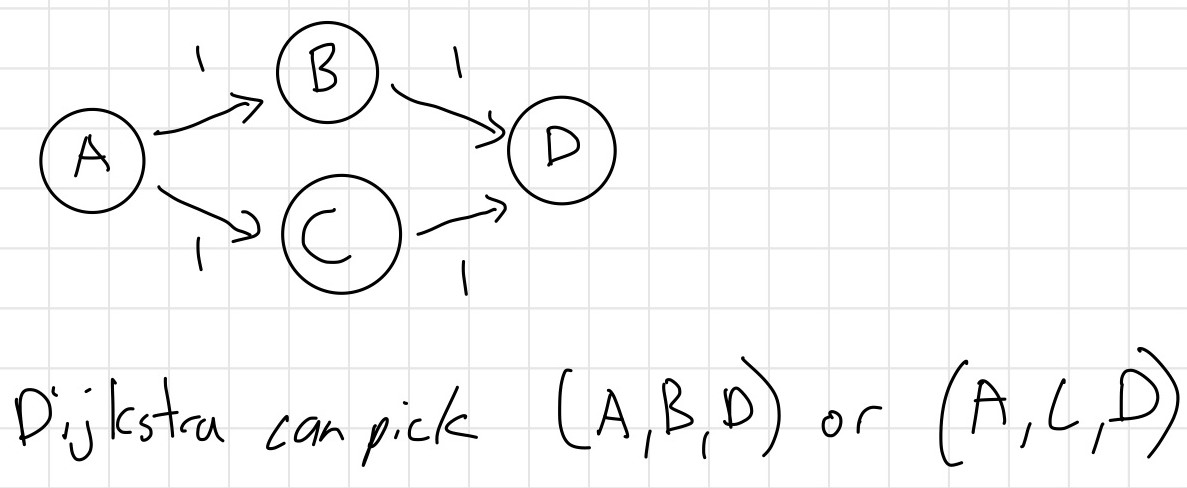
\includegraphics[width=0.75\textwidth]{Dijkstra}
        \begin{proof}
            Assume by contradiction that Dijkstra's algorithm picks a different set of edges
            after doubling the weights of the edges.\newline
            Let $\mathbb{D}$ be the set of edges picked by Dijkstra's algorithm before doubling
            the weights of the edges, we'll denote its weight as $W_{D}$.\newline
            Let $\mathbb{D'}$ be the set of edges picked by Dijkstra's algorithm after doubling
            the weights of the edges, we'll denote its weight as $W_{D'}$.\newline
            Assume $\mathbb{D'} \neq \mathbb{D}$.\newline
            Since Dijkstra's algorithm picks the path with the minimum weight, then $W_{D'} \leq
            2 \cdot W_{D}$.\newline
            Then, since $W_{D'}$ is the total weight of the doubled edges, then the total weight
            of the path before doubling the edges is $W_{D'} / 2$.\newline
            Using the previous inequality, this implies $W_{D'} / 2 \leq W_{D}$.\newline
            Since $W_{D}$ is the minimum weight of the path, then $W_{D'} / 2 = W_{D}$.\newline
            Then, $\mathbb{D'}$ has the same path weight as $\mathbb{D}$.\newline
            Now, we show that $\mathbb{D'}$ has the same edges as $\mathbb{D}$.\newline
            Assume by contradiction that $\mathbb{D'}$ has a different set of edges than
            $\mathbb{D}$.\newline
            Let the first differing edge be $(u, v)$ in $\mathbb{D}$.\newline
            Then, the weight of the path from the source to $u$ in $\mathbb{D'}$ = $2 \cdot \mathbb{D}$.\newline
            Then, since Dijkstra's algorithm picks the path with the minimum weight, then that
            means $\mathbb{D'}$ found a cheaper edge.\newline
            However, since $(u, v)$ is the cheapest edge in $\mathbb{D}$, then $\mathbb{D'}$
            should have picked it since after doubling it retains the quality of being the cheapest
            .\newline
            This is a contradiction, so $\mathbb{D'}$ has the same set of edges as $\mathbb{D}$
            .\newline
            $\therefore$, Dijkstra's algorithm picks the same set of edges after doubling the
            weights of the edges.
        \end{proof}
    \end{homeworkProblem}

\end{document}
%%% Local Variables:
%%% mode: latex
%%% TeX-master: t
%%% End:
